\chapter{Emscripten}
\label{cha:emscripten}

JavaScript is often called an assembly language of the Web.\footnote{http://www.hanselman.com/blog/JavaScriptIsWebAssemblyLanguageAndThatsOK.aspx} One could argue that since only one language is supported by browsers it could be made a compilation target similar to assembler for CPU. This statement is flawed since eventually JavaScript is translated to assembly making it only an intermediate step. Probably resemblance to ByteCode in JVM, which is compilation target of multiple languages like Java, Scala and Clojure is more in place.
Nevertheless, last years showed multiple projects aimed at converting code to JavaScript. Some introduce new syntax like CoffeeScript, Dart or TypeScript while still serving the same purpose - providing human readable code that is interpreted in browser on fly. Others, that are focus of this chapter, aim to convert existing projects to run in browser.

Several new projects are connected to make this happen. First steps in conversion between languages were made with LLVM project\footnote{http://llvm.org/} which currently is a collection of tools and compilers converting code to and from intermediate representation (LLVM IR). For C++ Clang\footnote{http://clang.llvm.org/} is a conversion tool.

\begin{figure}[h!]
  \caption{Pipeline of Emscripten conversion. Source: http://www.hanselman.com/blog/JavaScriptIsWebAssemblyLanguageAndThatsOK.aspx}
  \label{img:emscriptenpipeline}
  \centering
	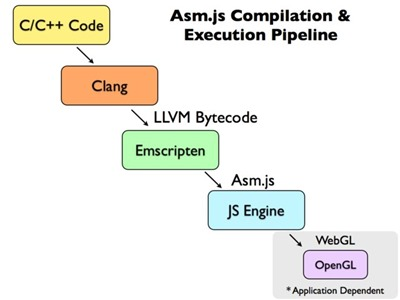
\includegraphics[width=8cm]{emscripten/pipeline.jpg}
\end{figure}

Code in LLVM is suitable for further conversion to language like JavaScript. This part is handled by Emscripten\footnote{https://github.com/kripken/emscripten/wiki} project. Initially compilation target for Emscripten was plain JavaScript. With recent developments asm.js\footnote{http://asmjs.org/spec/latest/} library was created. It provides syntax built on top of JavaScript, that is strongly typed and easily translatable to assembly language. Asm.js details are explained in section \ref{sec:asmjsoverview}.

\lstinputlisting[caption=Example of code using asm.js,label=listing:asmjs]{emscripten/asm.js}

Project, built in cooperation with Mozilla Foundation, has its own engine for Firefox - OdinMonkey, designed to run faster for this limited and well-defined syntax.

Altogether these projects resulted in multiple libraries and games converted from native version to JavaScript.

Proof-of-concept demo made in cooperation between Mozilla and Unreal is Epic Citadel HTML5 - Unreal Engine 3 technology demo\footnote{http://www.unrealengine.com/en/showcase/udk/epic\_citadel/}  instance running in browser.\footnote{http://www.unrealengine.com/html5/} Companies claim it took only four days to complete the conversion.

\begin{figure}[h!]
  \caption{Epic Citadel screenshot}
  \label{img:epicitadel}
  \centering
	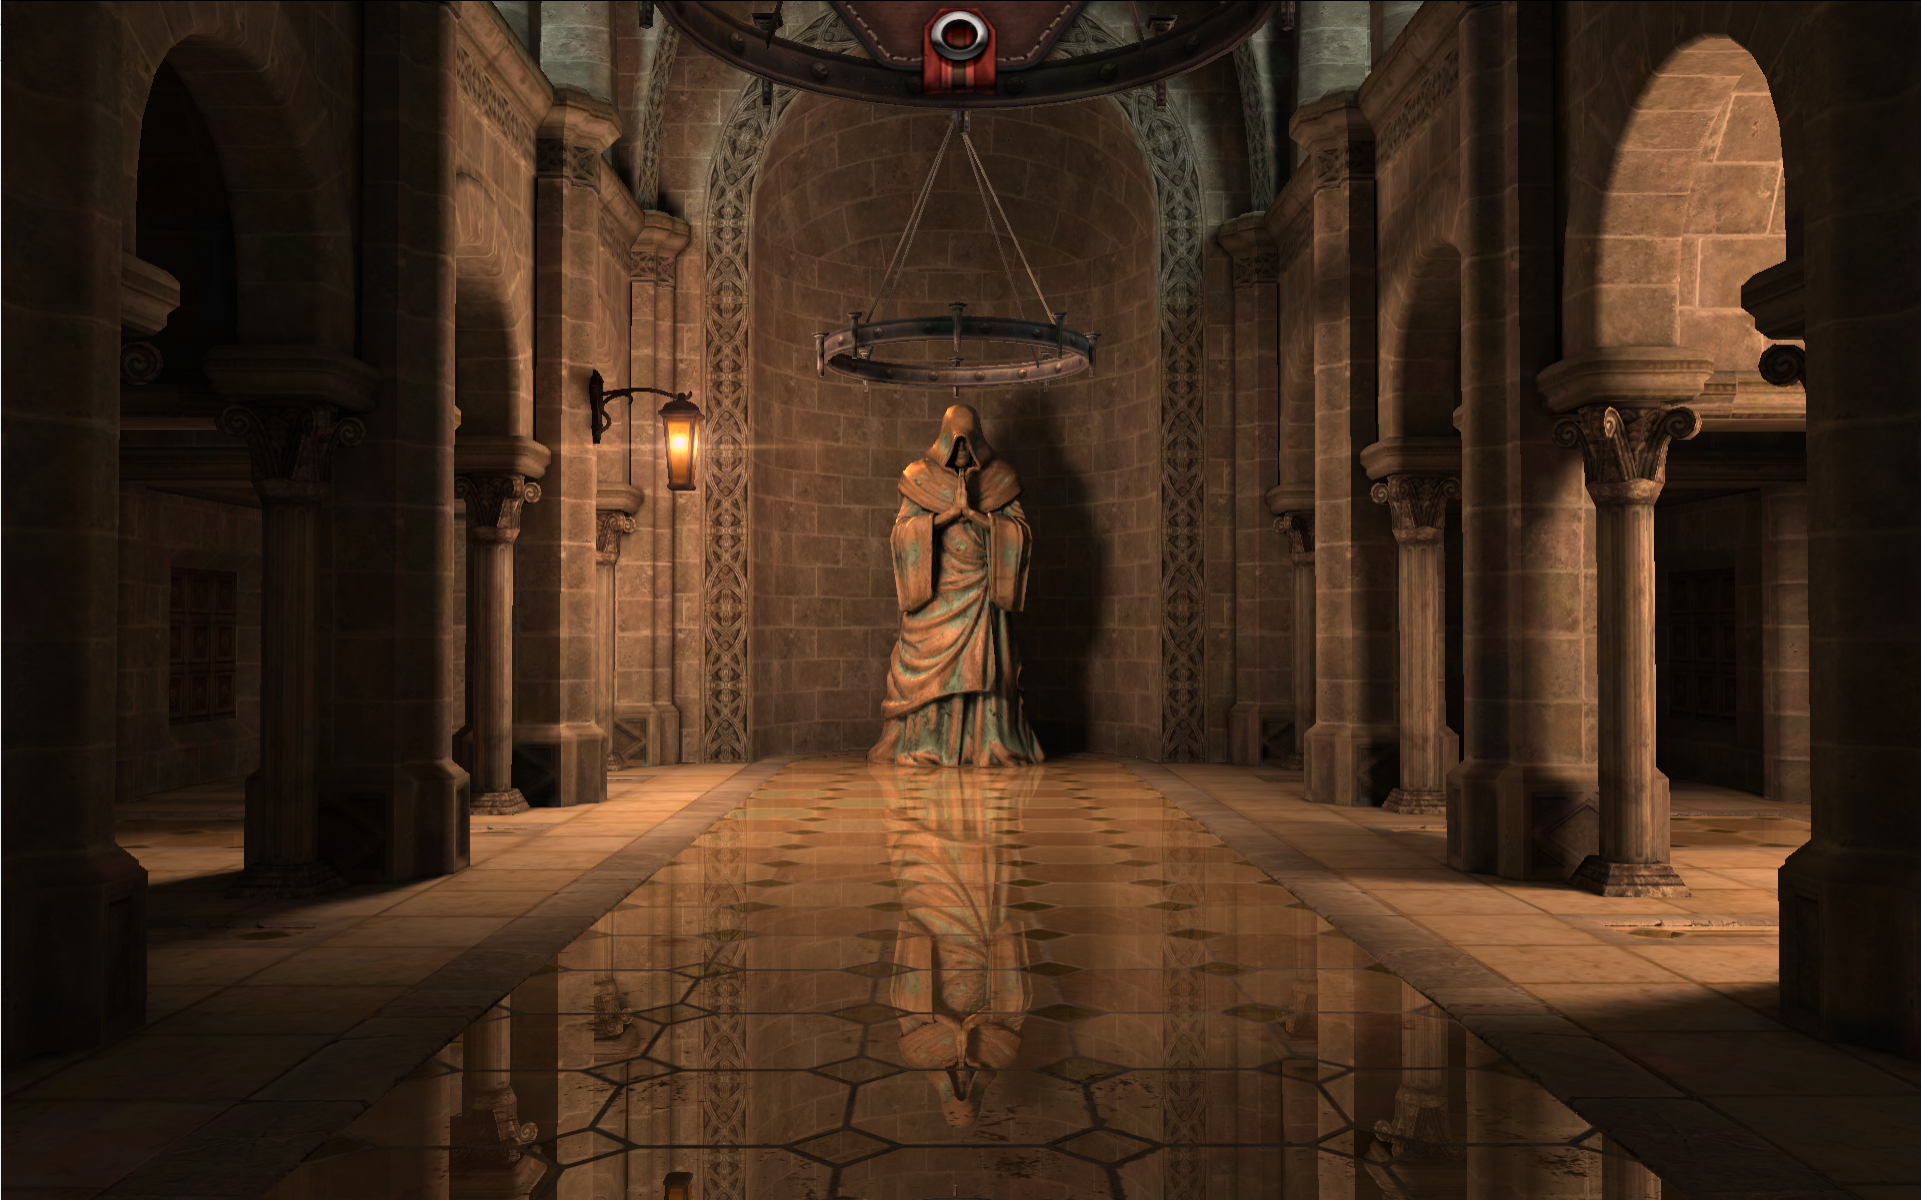
\includegraphics[width=16cm]{emscripten/epic-citadel.jpg}
\end{figure}

Another example of successful converted project is ammo.js\footnote{https://github.com/kripken/ammo.js/} - originating from Bullet physics engine.
TODO: Maybe extend this part a bit, cover more on how conversion was going and what were the issues.

\begin{figure}[h!]
  \caption{Ammo.js demo colliding 500 boxes at 30fps, available at http://kripken.github.io/ammo.js/examples/new/ammo.html}
  \label{img:epicitadel}
  \centering
	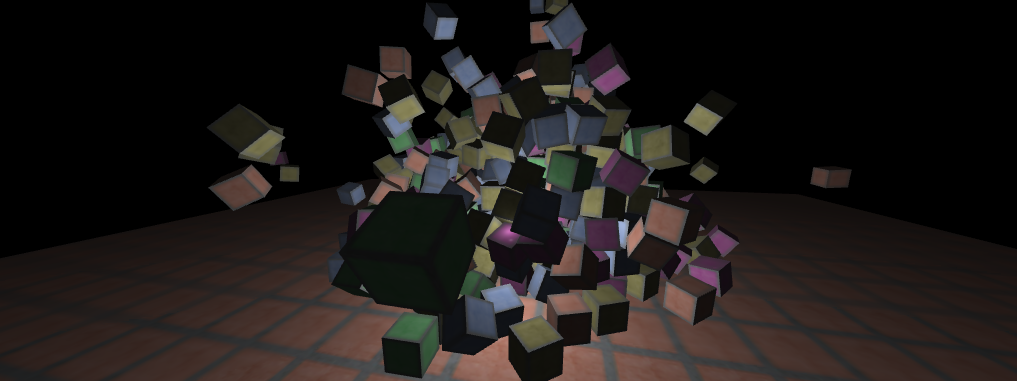
\includegraphics[width=16cm]{emscripten/ammojs.png}
\end{figure}

\section{Asm.js overview}
\label{sec:asmjsoverview}

Asm.js introduces some improvements targeted to fix performance problems of JavaScript. Ahead of time compilation enforces very specific rules on coding style. Documentation\footnote{http://asmjs.org/spec/latest/} lists:

\subsection{Unboxed representations of integers and floating-point numbers}
\label{sec:asmjsunboxed}
In asm.js only types allowed are integers and doubles. All numbers have annotations indicating static type (see: \ref{listing:typestree}). This way compiler doesn't have to detect possible transitions between variable types and code overall runs faster.

\subsection{Absence of runtime type checks}
\label{sec:asmjstypechecks}
Since asm.js works only on well-defined numbers, all function calls are monomorphic and stable. In OdinMonkey ahead-of-time compilation is able to compile them to the most optimised version without tracking method calls. In engines using JIT methods are compiled early and newer deoptimised.

\subsection{Absence of garbage collection}
\label{sec:asmjsgc}
As shown in previous chapters, garbage collection calls are often a performance bottleneck. Asm.js solves this problem by eliminating garbage collection completely. Memory is stored in short-life variables, deallocated after method exits and in global heaps, which are never resized or deallocated.

\subsection{Efficient heap loads and stores}
\label{sec:asmjsheap}

Heaps are global arrays of statically typed arrays, in JavaScript implemented as objects listed in \ref{table:jsarrays}. Size of heap doesn't change during runtime - it has to be calculated during compilation and incorrect prediction or memory leaks may result in buffer overflow. Heaps are always passed as an argument to asm.js modules. Each module may reference part of the heap and use it as long as necessary.

\begin{table}[h!]
\caption{Statically typed arrays in JavaScript}
\centering
\label{table:jsarrays}
\begin{tabular}{|l|l|l|}
  	\hline
View Type & Element Size (Bytes) & Element Type \\ \hline
Uint8Array & 1 & intish \\ \hline
Int8Array & 1 & intish \\ \hline
Uint16Array & 2 & intish \\ \hline
Int16Array & 2 & intish \\ \hline
Uint32Array & 4 & intish \\ \hline
Int32Array & 4 & intish \\ \hline
Float32Array & 4 & doublish \\ \hline
Float64Array & 8 & doublish \\ \hline
\end{tabular}
\end{table}

\subsection{Summary}
\label{sec:asmjssummary}

These solutions remove some of performance bottlenecks described in previous chapters. Code suitable to run with asm.js is almost unreadable by programmer and resembles assembly code. Asm.js is not designed to be a language used by a programmer, it is mainly a target for compilation using converters like Emscripten. 

Most of optimisation used by asm.js are consistent with code that is expected by V8 engine - variables and methods are monomorphic, garbage collection is close to zero. It's worth noting that code written by hand is almost always shorter that one generated by Emscripten. Partial solution for this is built-in Google Closure Compiler used on output of Emscripten and different levels of optimisation.
In tests mentioned in this work all solutions take 2 to 4kB compiled, while Emscripten produces over 450kB of code for each. This affects real life performance by lengthening at least transfer and parse time for code. Average parse time of 1kB of JS is believed to be up to 1ms\footnote{https://developers.google.com/speed/docs/best-practices/mobile}. Global average bandwidth was 3.1 Mbps in Q1 2013\footnote{http://www.akamai.com/dl/akamai/akamai\_soti\_q113.pdf} thus transfer of each kilobyte is around 2.5ms. In total, load time of tested code is approximately 1.5 second on average bandwidth and platform. In case of larger applications and games waiting time for load may be significantly larger and should be taken under consideration.

\section{Benchmarks}
\label{sec:embenchmarks}

All four test were compiled and run times were measured on different platforms.

Unoptimised version of particle system (see: \ref{sec:particlesinitial}) were designed to perform a lot of memory operations. In tests it's visible that C++ handles this task best. Code generated using Emscripten benefits from static memory heap which effectively works similar to object pool introduced later and runs approximately twice as long as C++. Plain JavaScript suffers greatly from memory allocation issues and unoptimised code, resulting in 6 times slower execution than C++.

Optimised particles (see: \ref{sec:particlesobjectpool}) with object pool and low garbage collection show how improvements of algorithm result in much faster JavaScript execution. It still takes twice as long to run particle system in V8, but Emscripten version takes three times longer than C++. Additional overhead of long and complex code is clearly visible and since JS code employs the same techniques that Emscripten uses automatically, there is no improvement in related areas. It's worth mentioning that unoptimised version of C++ particle system is slightly slower than optimised JavaScript one, showing that code quality improvement that doesn't affect algorithmic complexity of algorithm may be more important than choice of environment.

\begin{table}[h!]
\caption{Particle tests on different platforms}
\label{table:benchmarks}
\begin{tabular}{|p{4cm}||l|l|l||l|l|l|}
  	\hline
   Platform & \multicolumn{3}{c}{Unoptimised particles} & \multicolumn{3}{c}{Optimised particles}\\ \hline
   & C++ & JavaScript & Emscripten & C++ & JavaScript & Emscripten\\ \hline
   Fedora 19, Intel i7 2670QM, 4GB RAM, g++ 4.8.1 & 3.21s & 19.51s & 4.85s & 1.63s & 4.96s & 5.10s \\ \hline
   Windows 7, Intel i7 2670QM, 4GB RAM, g++ 4.7.3, Cygwin & 3.51s & 20.77s & 6.46s & 1.71s & 3.47s & 5.57s \\ \hline
\end{tabular}
\end{table}

Sphere collision test is putting high load on CPU. 

In $O(n^2)$ version (see: \ref{sec:sphereinitial}) exactly 1 000 000 000 checks for object collisions are made. Overall execution time is surprisingly good for JavaScript with overhead of approximately 15\% and 25\% for Emscripten generated version. It's a result of putting focus on pure mathematical operations that are quickly compiled by V8 and processed on unboxed numbers in asm.js.

Space partitioning using Octree greatly reduces number of collisions (to less than 100 000) and execution time. To give meaningful results simulation time is increased from 1000 frames to 10000. Under these circumstances difference in run time changes to 20\% for Javascript and stays similarly around 25\% for Emscripten. This is result of small memory operations related to Octree areas.

\begin{table}[h!]
\caption{Spheres tests on different platforms}
\label{table:benchmarks}
\begin{tabular}{|p{4cm}||l|l|l||l|l|l|}
   \hline
   Platform & \multicolumn{3}{c}{$O(n^2)$ spheres} & \multicolumn{3}{c}{Octree spheres}\\ \hline
   & C++ & JavaScript & Emscripten & C++ & JavaScript & Emscripten\\ \hline
   Fedora 19, Intel i7 2670QM, 4GB RAM, g++ 4.8.1 & 4.96s & 9.02s & 12.35s & 
3.44s & 14.14s & 11.20s \\ \hline
   Windows 7, Intel i7 2670QM, 4GB RAM, g++ 4.7.3, Cygwin & 9.52s & 10.81s & 11.82s & 14.10s & 16.95s & 17.79s \\\hline
\end{tabular}
\end{table}

Above results show how well written JavaScript or properly converted C++ are able to perform in browser with similar performance as native programs, rarely exceeding 100\% overhead and sometimes getting as close as 15\% to C++ execution time. 
